\documentclass[14pt]{extarticle}

\let\Overrightarrow\overrightarrow
\let\vecarrow\overrightarrow


%other%
\usepackage{graphicx}
\usepackage{float}
\usepackage[margin=0.6in]{geometry}
\usepackage{caption}
\usepackage{csquotes}
\usepackage[export]{adjustbox}
\usepackage{wrapfig}
\usepackage{setspace}
\usepackage{anyfontsize}
\usepackage{titlesec}
\titleformat{\section}{
	\normalfont\fontsize{20}{20}\bfseries}{\thesection}{1em}{}
\titleformat{\subsection}{
	\normalfont\fontsize{17}{20}\bfseries}{\thesubsection}{0.1em}{}
\usepackage{relsize}
%other%



%%\newcommand{\F}{\Oldmathbfcal{F}}
%math%
\usepackage{amsthm}
\usepackage{amssymb}
\usepackage{amsmath}
\usepackage{mathtools}
%%\usepackage[cal = pxtx, scr = dutchcal]{mathalfa}



%\usepackage{unicode-math}
%\newtheorem*{}{\textup{Лемма}}
\newtheorem*{theorem}{\textup{Теорема}}
\newtheorem*{remark}{\textup{Комментарий}}
%\renewcommand\qedsymbol{$\blacksquare$}
%\usepackage{parskip}

\usepackage{pgfplots}
\usepgfplotslibrary{polar}
\usepgflibrary{shapes.geometric}
\usetikzlibrary{calc}


\renewenvironment{proof}
    {\noindent \textit{Доказательство.}\\
	\indent $\square$}
	{ $\blacksquare$\\ }

\newenvironment{solution}
	{\vspace{-4.3mm} \noindent\textbf{Решение.}}


\renewenvironment{remark}
    {\noindent\textbf{Коментарий}}

\usepackage{tikz}
   \usetikzlibrary{calc}

\newcommand{\arc}[0]{
   \tikz [baseline = (N.base), every node/.style={}] {
	  \node [inner sep = 0pt] (N){}; %{$#0$};
      \draw [line width = 0.8pt] plot [smooth, tension=1.3] coordinates {
         ($(N.north west) + (-1.5ex,0.6ex+0.4ex)$)
         ($(N.north)      + (-0.75ex,0+0.4ex)$)
         ($(N.north east) + (0ex,0.6ex+0.4ex)$)
      };
   }
}

\renewenvironment{rcases}
  {\left.\begin{aligned}}
  {\end{aligned}\right\rbrace}

\DeclarePairedDelimiter\abs{\lvert}{\rvert}
\DeclarePairedDelimiter\norm{\lVert}{\rVert}

%\newcounter{example}[section]
\newenvironment{example}[1]{\noindent \textbf{Пример #1.}}

\let\mathb\mathbb


\newcommand{\N}{\mathb{N}}
\newcommand{\Z}{\mathb{Z}}
\newcommand{\R}{\mathb{R}}
\newcommand{\F}{\mathbfcal{F}}
\renewcommand{\P}{\mathbfcal{P}}
%\newcommand*{\Z}{\mathbb{Z}}
%math%

%fonts%
%%\usepackage[russian]{babel}
%\usepackage{polyglossia}
%\setdefaultlanguage[spelling=modern]{russian}
%\setotherlanguage{english}
%\setmainfont{CMU Serif}
%\setsansfont{CMU Sans Serif}
%%\setmonofont{CMU Typewriter Text}  
%\setmathfont{Latin Modern Math}
\usepackage{mathrsfs}
%\DeclareMathAlphabet{\mathcal}{T1}{TX}{m}{n}

\usepackage{unicode-math}


%\let\Oldmathbfcal=\mathbfcal
%\renewcommand{\mathbfcal}{\mumble\Oldmathbfcal}

%%\newcommand{\F}{\Oldmathbfcal{F}}
%%\newcommand{\F}{𝓕}

%\usepackage{fontspec}
\setmathfont{Latin Modern Math}

\DeclareSymbolFont{symbols}{OMS}{cmsy}{m}{n}
\DeclareSymbolFont{bsymbols}{OMS}{cmsy}{b}{n}
\DeclareSymbolFontAlphabet{\mathcal}{symbols}
\DeclareSymbolFontAlphabet{\mathbfcal}{bsymbols}

%\setmathfont[range = {2131}]{AMS}
%\usepackage{amsfonts}
%\usepackage{dsfont}

\begin{document}
\textbf{Problem.} Consider a points \(B\) and \(C\), lying inside the given 
angle \(ASD\), such that \(\angle BSA = \angle CSD\). Lines \(BD\) and 
\(AC\) meet at \(Q\) and lines \(AB\) and \(CD\) meet at \(P\). 
It turns out, that quadrilateral \(BPCQ\) has inscribed circle 
\(\omega\). Prove that center \(I\) of \(\omega\) 
lies on the angle bisector of angle \(\angle ASD\). 
(Author -- Nikita Kolesnikov) 

\textbf{Solution.}

\begin{figure}[H]
    \centering
    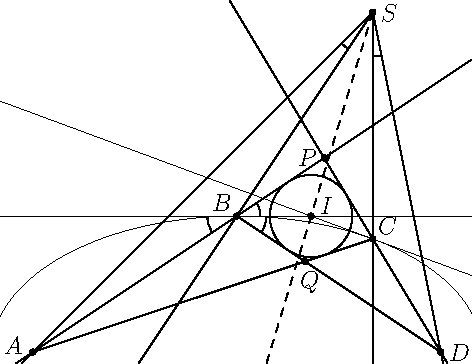
\includegraphics[height=8cm]{fig.pdf}
\end{figure}

Let me remind you, that there exists an ellipse \(\P\) with focuses 
\(A\) and \(D\), passing through points \(B\) and \(C\). It's easy 
to see, that tangents to ellipse \(\P\) at points \(B\) and \(C\) are the 
angle bisectors of angles \(\angle PBQ\) and \(\angle QCP\) respectively.
(it can be obtainted by applying optical property of ellipse to these 
tangents)

Let \(\ell\) be the angle bisector of angle \(\angle ASD\). So it suffices to prove, that tangents to \(\P\) at \(B\) and at \(C\) 
intersect on \(\ell\).
\begin{figure}[H]
    \centering
    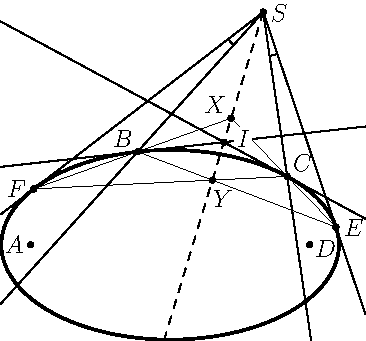
\includegraphics[height=9cm]{fig2.pdf}
\end{figure}

Let \(E\) and \(F\) be the points on \(\P\) such that \(SE\) and \(SF\) 
are tangents to the ellipse \(\P\). Since 
\(\angle FSA = \angle ESD\) (isogonal property of ellipse) and 
\(\angle ASB = \angle DSC\) it follows that \(\angle FSB = \angle ESC\).
Let \(X\) be the intersection point of lines \(FB\) and \(CE\). 
Let \(Y\) be the intersection point of lines \(BE\) and \(CF\). 
Applying Isogonal's theorem (to the points \(F\), \(B\), \(C\), \(E\)), 
we get \(\angle FSX = 
\angle ESY\). On the other hand, Pascal's theorem for quadrilateral 
\(FBCE\), gives us that \(S\), \(X\), \(Y\), \(I\) are collinear. Since 
\(\angle FSX = \angle ESY\) this implies that \(X\) and \(Y\) lies 
on \(\ell\). It follows that \(I\) also lies on \(\ell\), as desired.

\end{document}
